\documentclass[a4paper,11pt]{scrartcl}
\usepackage[T1]{fontenc}
\usepackage[utf8]{inputenc}
\usepackage[ngerman]{babel}
\usepackage{babelbib}

\usepackage[a4paper]{geometry}
\usepackage{amsmath}

\usepackage{listings}

% Ermöglicht Fußnoten in gleitenden Umgebungen
\usepackage{footnote}


\pdfminorversion=6

\usepackage{eurosym}  % € Zeichen
\usepackage{nicefrac} % Einhalbzeichen
\usepackage{url}      % URLs
\usepackage{breakurl} % break urls
\usepackage[perpage,bottom,marginal]{footmisc} % Footnote configuration

\usepackage{hyperref}
\hypersetup{
  colorlinks  = false,     % don't color links
  pdfborder   = {0 0 0},    % don't put stupid rectangles around links
  pdftitle    = {Softwareprojektbericht: Common Unfolding},
  pdfsubject  = {Bericht und Dokumentation zum Softwareprojekt Common Unfolding},
  pdfauthor   = {Alexa Schlegel, Friedrich Keinhorst, Henry Dettmer},
  pdfstartview= FitH,
  pdfkeywords = {Softwareprojekt, Bericht, Dokumentation, 2011, Sommersemester}]
}

% für die Grafiken
\usepackage{graphicx}

% mehrer Grafiken nebeneinander
\usepackage[hang]{subfigure}

% vertikalen Abstand anstelle von horizontalem Abstand bei Absätzen
\setlength{\parskip}{\smallskipamount}
\setlength{\parindent}{0pt}

%für Kommentare
\usepackage{verbatim}

% Rotation der Tabelle
\usepackage{rotating}
\usepackage{booktabs} 
\renewcommand{\arraystretch}{1.2}
\usepackage{arydshln}

%Captions von Bildern, Tabellen usw.
\usepackage[labelfont=bf]{caption} 
\setlength{\belowcaptionskip}{0.3cm}

%Seitenheaders
\usepackage{fancyhdr}

% Beschriftung in Bildern
\usepackage[svgnames]{pstricks}
\usepackage{pst-text}
\definecolor{bg}{cmyk}{0,0,0.1,0}

\usepackage[page,titletoc]{appendix} % appendix in toc

\newcommand{\goodgap}{%
\hspace{\subfigtopskip}%
\hspace{\subfigbottomskip}}


\newcommand\parbig{\par\bigskip}

%TYPORGAPHISCHES
\usepackage{xspace}
\newcommand{\zB}{\mbox{z.\,B.}\xspace}
\newcommand{\bzw}{\mbox{bzw\!.}\xspace}
\newcommand{\usw}{\mbox{usw\!.}\xspace}
\newcommand{\dH}{\mbox{d.\,h.}\xspace}
\newcommand{\mailto}[1]{\href{mailto:#1}{#1}}

% Keine Ahnung warum, aber "`bla"' funktioniert bei mir nicht.
\newcommand{\enquote}[1]{\glqq{}#1\grqq{}}

% Abstract
\renewcommand{\abstractname}{Zusammenfassung}

%URLPROBLEM
\urldef{\makro}{\url}{http://javascriptmvc.com/docs.html#!jQuery.fn.selection}

% DECKBLATT
% Titel and author 
\title{
  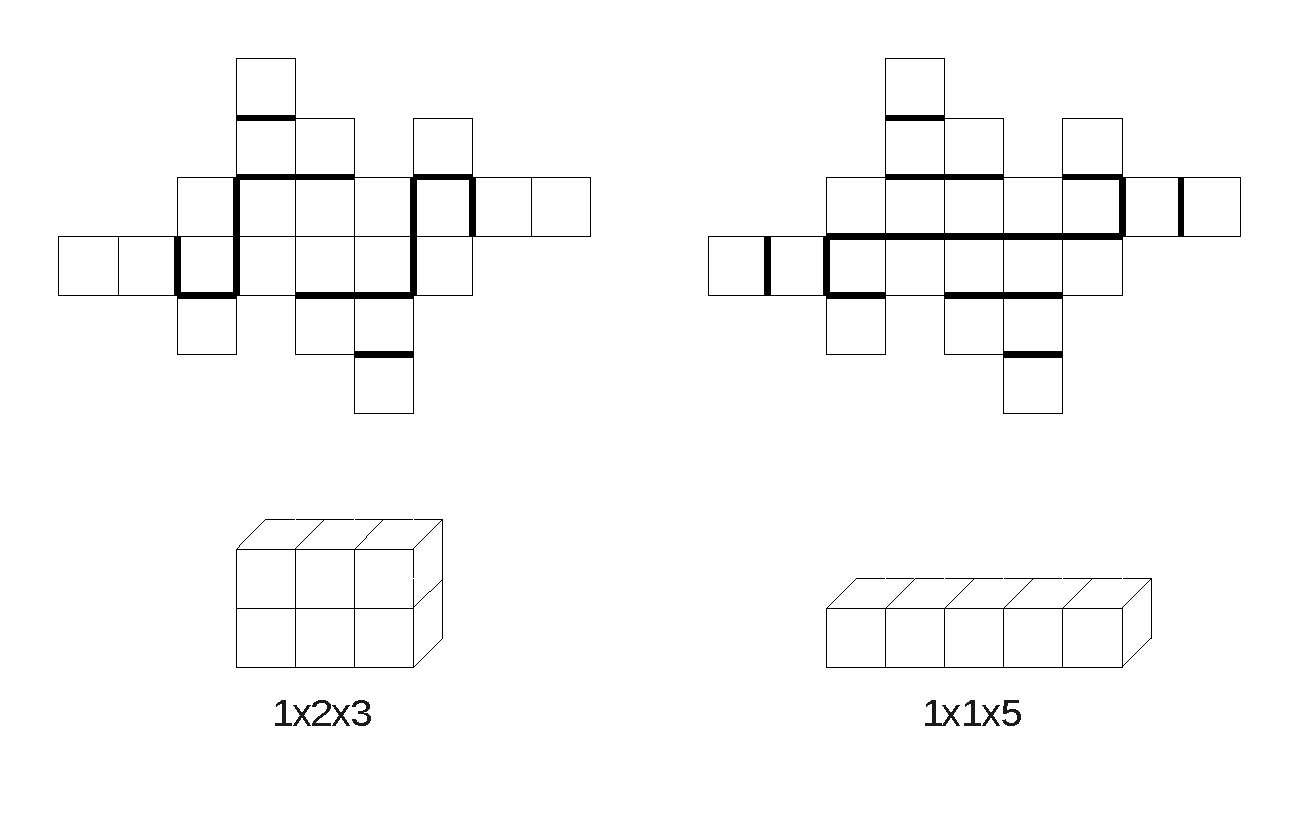
\includegraphics[width=0.6\textwidth]{03_pics/commonUnfold_beispiel1.pdf}\\
  [4ex]
  {
  \normalsize Softwareprojekt über Anwendung von Algorithmen\\
  [2ex]
  }
  Abschlussbericht zum Softwareprojekt\\
  \enquote{Common Unfolding}\\
  [4ex]
  {\normalsize Sommersemester 2011}\\
  {\normalsize Betreuer: Prof. Dr. Rote}\\
  [4ex]
}

\author{Alexa Schlegel\\\mailto{alexa.schlegel@gmail.com} \and Friedrich Keinhorst\\\mailto{fkeinhorst@gmail.com} \and Henry Dettmer\\\mailto{henrydettmer@gmail.com}\\[4ex]
}

\date{Berlin, \today}


\hyphenation{}

\begin{document}

\begin{titlepage}

\pagenumbering{alph}
\maketitle
\thispagestyle{empty}

\vfill{}
\end{titlepage}

\pagestyle{empty}
\clearpage\pagenumbering{roman}

\tableofcontents
\clearpage

\pagenumbering{arabic}
\pagestyle{fancy}
\setcounter{page}{1}

\begin{abstract}
Gegenstand des Projektes, Zielstellung, Umsetzung, Ergebnis, Am Ende
schreiben.
\end{abstract}
\clearpage


\section{Einleitung}
\label{sec:einleitung}

Das Softwareprojekt \emph{Common Unfolding} entstand im Sommersemester 2011 im Rahmen der Veranstaltung \emph{Softwareprojekt: Anwendungen von Algorithmen} unter Leitung von Herrn Prof. Dr. Rote. Es entstand ein Programm, mit dessen Hilfe, auf zeichnerischem Wege Polygone gefunden werden können, aus denen zwei verschieden Quader \bzw Schachteln gefaltet werden können. Im Folgenden wird die genaue Problemstellung näher erläutert, sowie die Zielstellung unseres Projektes definiert.


%%%%%%%%%%%%%%%%%%%%%%%%%%%%%%%%%%%%%%%%%%%%%%%%%%%%%%%%%%%%%%%%%%%%%%%%%%%%%%%
%%%%%%%%%%%%%%%%%%%%%%%%%%%%%%%%%%%%%%%%%%%%%%%%%%%%%%%%%%%%%%%%%%%%%%%%%%%%%%%
%%%%%%%%%%%%%%%%%%%%%%%%%%%%%%%%%%%%%%%%%%%%%%%%%%%%%%%%%%%%%%%%%%%%%%%%%%%%%%%
% PROBLEMSTELLUNG UND AUFGABENSTELLUNG %%%%%%%%%%%%%%%%%%%%%%%%%%%%%%%%%%%%%%%%
%%%%%%%%%%%%%%%%%%%%%%%%%%%%%%%%%%%%%%%%%%%%%%%%%%%%%%%%%%%%%%%%%%%%%%%%%%%%%%%
\subsection{Problemstellung und Aufgabenstellung}
\label{subsec:problemstellung}

Grundsätzlich geht es um das Falten von orthogonalen Polygonen zu Quadern \bzw Schachteln. Unter orthogonalen Polygonen versteht man Polygone, die ausschließlich Innenwinkel mit 90$^\circ$ oder 270$^\circ$ besitzen. Beispielsweise ist das Netz eines Würfles ein orthogonales Polygon (siehe Abb.~\ref{fig:polygon}).

\begin{figure}[htbp]
\centering
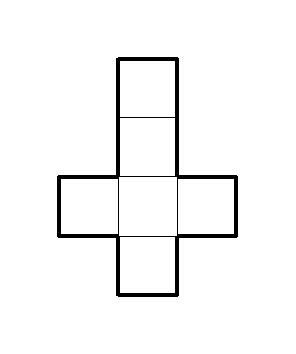
\includegraphics{03_pics/polygon.pdf}
\caption{Orthogonales Polygon}
\label{fig:polygon}
\end{figure}

Es existieren orthogonale Polygone als Grundfläche, welche, auf unterschiedliche Arten, \dH an verschiedenen Kanten gefaltet, in zwei verschieden dimensionierten Quadern resultieren. Dieses Polygon wird als \emph{common unfolding}~\cite{commonUnfold} der Quader bezeichnet. In Abbildung \ref{fig:Common-Unfolding} ist ein Beispiel einer Grundfläche gezeigt, aus welcher zwei verschiedene Schachteln in den Dimensionen $1\times2\times3$ und $1\times1\times5$ gefaltet werden können. Da beide Schachteln aus dem selben Polygon gefaltet wurden, haben sie identische Oberflächeninhalte.

\begin{figure}[htbp]
\centering
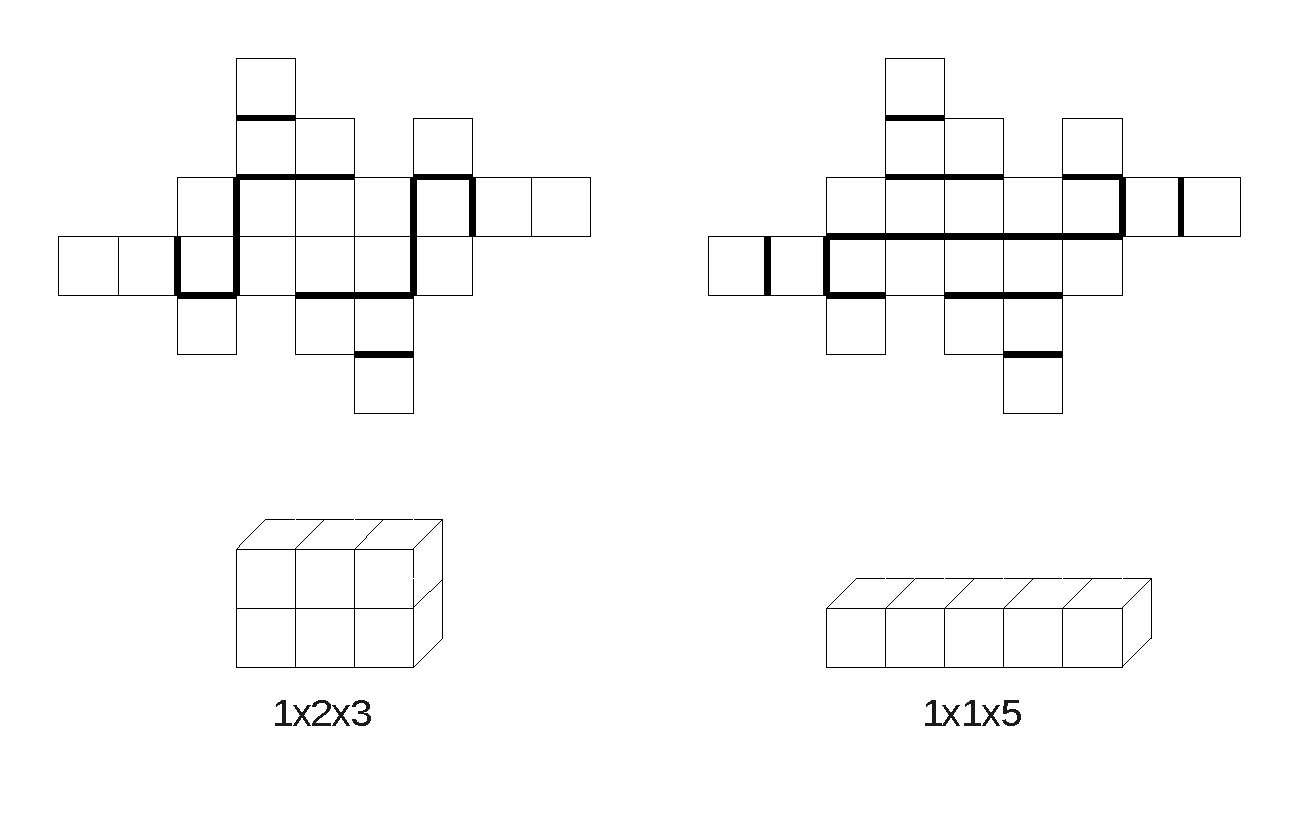
\includegraphics[scale=0.5]{03_pics/commonUnfold_beispiel1.pdf}
\caption{Common Unfolding}
\label{fig:Common-Unfolding}
\end{figure}

Um solche Grundflächen (common unfoldings) zu finden, war es unsere Aufgabe ein Programm zu entwickeln, welches eine zeichnerische Lösung des Problems ermöglicht. Zur Lösungsfindung wird die Idee des \emph{Simultanen Zeichnens} verwendet. Unter simultanem Zeichnen versteht man das gleichzeitige Zeichnen auf mehreren Grundflächen \bzw aufgefalteten Gitternetzen, siehe Abbildung~\ref{fig:Simpultanes-Zeichnen}. Ausgangspunkt sind dabei zwei (oder mehr) Quader mit verschiedenen Kantenlängen, aber gleichem Flächeninhalt. Für diese Quader soll nun, falls existent, das common-unfold Polygon gefunden werden. Auf den Oberflächen der Quader, wird gleichzeitig gezeichnet. Genauer gesagt ist die Oberfläche der Quader in beliebig kleine Flächenstücke eingeteilt, welche \emph{ausgemalt} werden. Wir erhalten die Lösung, wenn alle gegeben Quaderoberflächen komplett ausgemalt sind. Die Stellen an denen die Schachtel gefaltet werden soll, muss selbständig gefunden werden, eine Lösung dafür wird durch das Programm nicht geliefert. 


\begin{figure}[htbp]
\centering
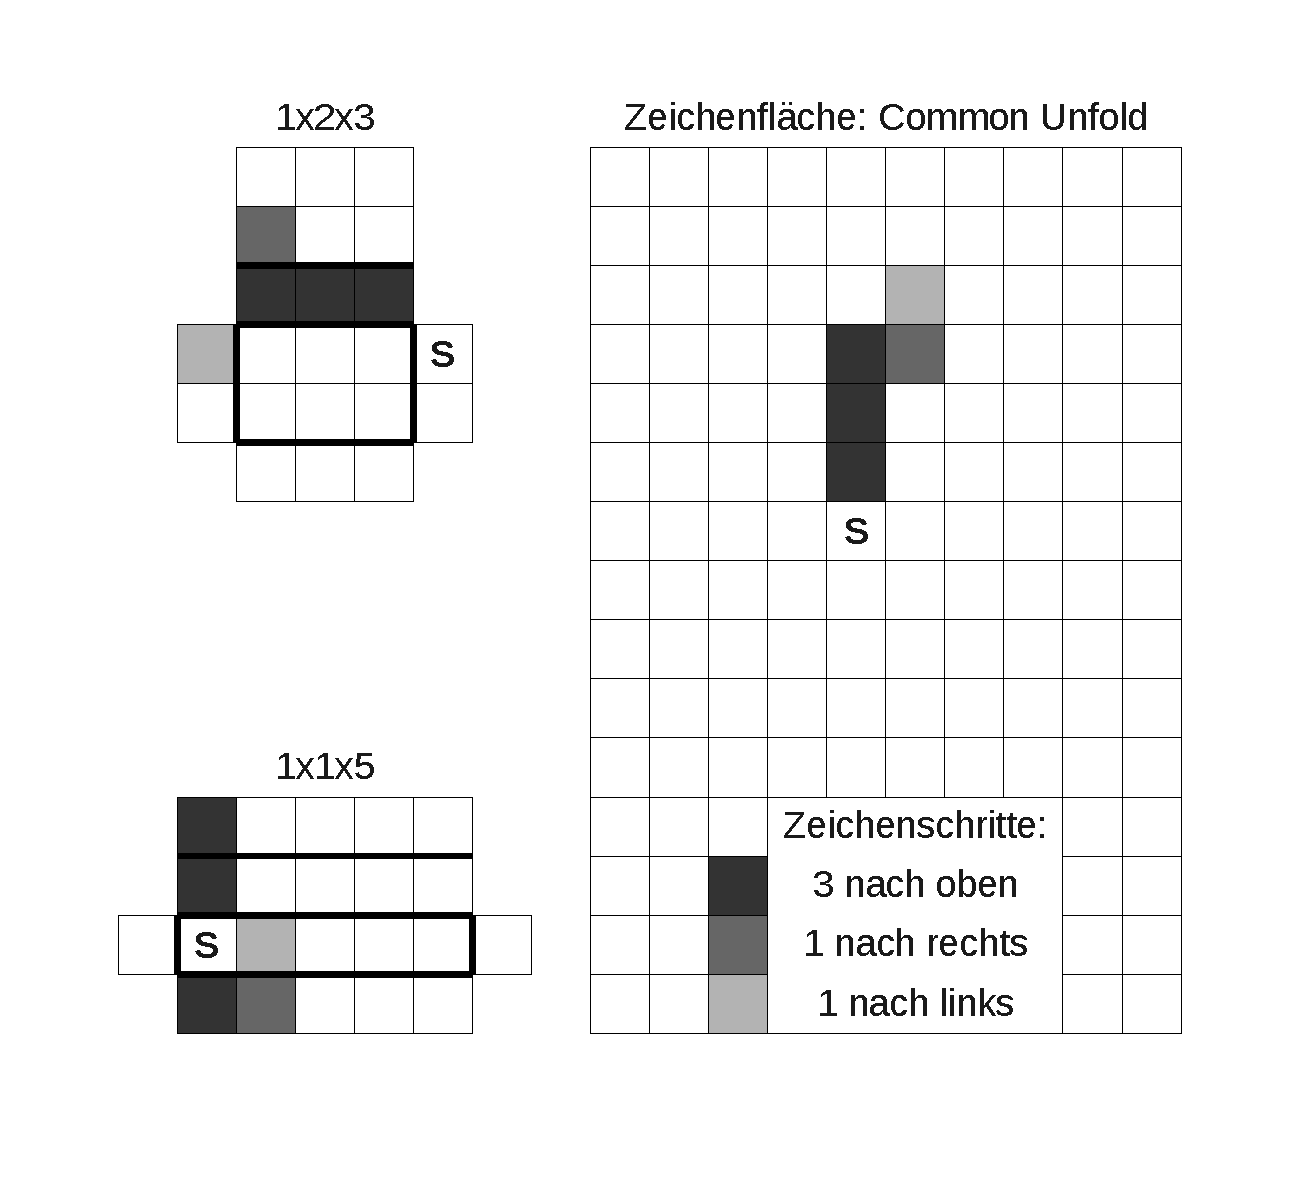
\includegraphics[scale=0.5]{03_pics/simulatnes_zeichnen.pdf}
\caption{Simpultanes Zeichnen}
\label{fig:Simpultanes-Zeichnen}
\end{figure}


%%%%%%%%%%%%%%%%%%%%%%%%%%%%%%%%%%%%%%%%%%%%%%%%%%%%%%%%%%%%%%%%%%%%%%%%%%%%%%%
%%%%%%%%%%%%%%%%%%%%%%%%%%%%%%%%%%%%%%%%%%%%%%%%%%%%%%%%%%%%%%%%%%%%%%%%%%%%%%%
%%%%%%%%%%%%%%%%%%%%%%%%%%%%%%%%%%%%%%%%%%%%%%%%%%%%%%%%%%%%%%%%%%%%%%%%%%%%%%%
% ZIELE UNSERES PROJEKTS %%%%%%%%%%%%%%%%%%%%%%%%%%%%%%%%%%%%%%%%%%%%%%%%%%%%%%
%%%%%%%%%%%%%%%%%%%%%%%%%%%%%%%%%%%%%%%%%%%%%%%%%%%%%%%%%%%%%%%%%%%%%%%%%%%%%%%
\subsection{Ziele unseres Projekts}
\label{subsec:ziele}

Das Ziel unseres Softwareprojektes war es, ein Programm zu entwickeln, welches eine 2D grafische Benutzeroberfläche bietet, um solche \emph{common unfolding}-Polygone zu finden. Das Programm sollte eine flexible Auswahl der Startquader bieten und den zeichnerischen Vorgang, also das gleichzeitige Zeichnen auf mehreren Schachtel ermöglichen.

\newpage


%%%%%%%%%%%%%%%%%%%%%%%%%%%%%%%%%%%%%%%%%%%%%%%%%%%%%%%%%%%%%%%%%%%%%%%%%%%%%%%
%%%%%%%%%%%%%%%%%%%%%%%%%%%%%%%%%%%%%%%%%%%%%%%%%%%%%%%%%%%%%%%%%%%%%%%%%%%%%%%
%%%%%%%%%%%%%%%%%%%%%%%%%%%%%%%%%%%%%%%%%%%%%%%%%%%%%%%%%%%%%%%%%%%%%%%%%%%%%%%
% GLIEDERUNG %%%%%%%%%%%%%%%%%%%%%%%%%%%%%%%%%%%%%%%%%%%%%%%%%%%%%%%%%%%%%%%%%%
%%%%%%%%%%%%%%%%%%%%%%%%%%%%%%%%%%%%%%%%%%%%%%%%%%%%%%%%%%%%%%%%%%%%%%%%%%%%%%%
\subsection{Gliederung der Arbeit}
\label{subsec:gliederung}
Der Abschlussbericht ist wie folgt strukturiert: Zunächst wird das Projektmanagement in Kapitel~\ref{sec:projektmanagement} erläutert. Dazu gehören die Erfahrungen bezüglich der Zusammenarbeit im Team und der Ablauf des Entwicklungsprozesses.\\

In Kapitel~\ref{sec:frontend} wird das User Interface und die Bedienung des Programms vorgestellt.\\

Eine Beschreibung der Anforderungen und Funktionalität des Programms, sowie der verwendeten \bzw implementierten Algorithmen und Funktionen erfolgt im Kapitel~\ref{sec:backend}: Softwarearchitektur. Dabei werden Schwierigkeiten und Herausforderungen bezüglich der Implementierung dargelegt und Verbesserungsmöglichkeiten aufgezeigt.\\

Schließlich erfolgt in Kapitel~\ref{sec:zusammenfassung} eine Zusammenfassung der Projektergebnisse und der erreichten Ziele. Außerdem werden unsere gewonnen Erkenntnisse \bzw "`Was haben wir dabei gelernt?"' dargelegt und ein Ausblick auf zukünftige Arbeiten gegeben.


\clearpage

\section{Projektmanagement}
\label{sec:projektmanagement}

Im Folgenden wird die Projektgruppe vorgestellt und die Zusammenarbeit im Team sowie die dabei entstandenen Herausforderungen und Schwierigkeiten erläutert. Auf die Auswirkungen der Teamarbeit auf den Entwicklungsprozess wird im Anschluss eingegangen. Es wird der geplante, sowie der letztlich umgesetzte Entwicklungsprozess mit Aufgabenverteilung und Zeitplan vorgestellt.

%%%%%%%%%%%%%%%%%%%%%%%%%%%%%%%%%%%%%%%%%%%%%%%%%%%%%%%%%%%%%%%%%%%%%%%%%%%%%%%
%%%%%%%%%%%%%%%%%%%%%%%%%%%%%%%%%%%%%%%%%%%%%%%%%%%%%%%%%%%%%%%%%%%%%%%%%%%%%%%
%%%%%%%%%%%%%%%%%%%%%%%%%%%%%%%%%%%%%%%%%%%%%%%%%%%%%%%%%%%%%%%%%%%%%%%%%%%%%%%
% TEAMMITGLIEDER %%%%%%%%%%%%%%%%%%%%%%%%%%%%%%%%%%%%%%%%%%%%%%%%%%%%%%%%%%%%%%
%%%%%%%%%%%%%%%%%%%%%%%%%%%%%%%%%%%%%%%%%%%%%%%%%%%%%%%%%%%%%%%%%%%%%%%%%%%%%%%
\subsection{Projektgruppe und Teamarbeit}
\label{subsec:teammitglieder}

Das Softwareprojekt wurde mit vier Teammitgliedern begonnen. Dazu gehörten Alexa, Friedrich, Henry und Michael. Kurz vor Abschluss des Semesters hat Michael die Gruppe verlassen.

Die Tatsache, dass wir uns alle nicht kannten, weder aus vorangegangenen Kursen noch privat, stellte eine große Herausforderung in der Teamarbeit dar. Die Einschätzung der Zuverlässigkeit und des Engagements, sowie der Programmierkenntnisse war dadurch schwierig. Wir hatten alle unterschiedliche Vorerfahrungen und bevorzugten unterschiedliche Programmiersprachen. Diese Punkte erschwerten zu Beginn des Projekts die Einarbeitung und die Aufgabenverteilung.

Da wir nur vier Leute im Team waren, haben wir uns dazu entschieden keinen Projektleiter zu bestimmen, jeder sollte gleichermaßen Verantwortung für das Projekt übernehmen.


%%%%%%%%%%%%%%%%%%%%%%%%%%%%%%%%%%%%%%%%%%%%%%%%%%%%%%%%%%%%%%%%%%%%%%%%%%%%%%%
%%%%%%%%%%%%%%%%%%%%%%%%%%%%%%%%%%%%%%%%%%%%%%%%%%%%%%%%%%%%%%%%%%%%%%%%%%%%%%%
%%%%%%%%%%%%%%%%%%%%%%%%%%%%%%%%%%%%%%%%%%%%%%%%%%%%%%%%%%%%%%%%%%%%%%%%%%%%%%%
% TEAMMITGLIEDER %%%%%%%%%%%%%%%%%%%%%%%%%%%%%%%%%%%%%%%%%%%%%%%%%%%%%%%%%%%%%%
%%%%%%%%%%%%%%%%%%%%%%%%%%%%%%%%%%%%%%%%%%%%%%%%%%%%%%%%%%%%%%%%%%%%%%%%%%%%%%%
\subsection{Entwicklungsprozess}
\label{subsec:prozess}

Wir haben uns für das Hosting des Projekts bei Spline\footnote{\url{https://dev.spline.de/trac/CommonUnfold/browser/trunk}} entschieden. Zur Codeversionierung wird dabei SVN verwendet. Zusätzlich verwenden wir einen Bug-Tracker\footnote{\url{https://dev.spline.de/trac/CommonUnfold/}}, welcher direkt von Spline zur Verfügung gestellt wurde.\\

Als Programmiersprache haben wir uns auf \emph{Python} geeinigt, da der vorgegebene Prototyp in Python implementiert war. Nur einer aus unserer Projektgruppe, Henry, war sehr sicher in Python, alle anderen mussten sich erst einmal in die neue Programmiersprache einarbeiten. Bevor wir mit der Implementierung anfingen, hatte jeder zwei Wochen Zeit sich in die neue Programmiersprache einzuarbeiten. Für die Programmierung der grafischen Oberfläche haben wir \emph{TkInter} verwendet, ein Wrapper des Tk-Toolkits für Python.\\

Wir haben uns für kein festes Vorgehensmodell zur Softwareentwicklung, wie beispielsweise das Wasserfallmodell, SCRUM oder TDD, entschieden. Um die Kommunikation im Team und unseren Prozess zu unterstützen, sowie um eine regelmäßige Arbeitsweise aller zu forcieren, haben wir uns für die folgenden Prozesselemente und Regeln entschieden:

  \begin{description}
    \item[Lauffähige Version im Repository] Um ein effektives Arbeiten zu ermöglichen, sollten nur lauffähige Versionen ins SVN committed werden.
    \item[Wöchentliche Treffen] Bei regelmäßigen, wöchentlichen Treffen (meist freitags 14:00 Uhr) haben wir über den aktuellen Stand und über neue Aufgaben gesprochen. Hier wurden Tickets eingetragen und Aufgaben direkt verteilt und zugewiesen.
    \item[Trac und Tickets] Die neuen Aufgaben, welche gemeinsam formuliert und besprochen wurden, wurden im Trac als Ticket gemeinschaftlich eingetragen. Das Trac-System war zentraler Bestandteil unserer Zusammenarbeit und wurde im Verlaufe des gesamten Projekts kontinuierlich verwendet.
    \item[Definierte Aufgaben pro Person] Jeder konnte sich Aufgaben aus den Tickets auswählen und sich verbindlich zuweisen. Jeder hatte dann für gewöhnlich ein oder zwei Aufgaben \bzw Tickets bis zum nächsten Treffen zu erledigen.
    \item[Aussagekräftige Commits] Aussagekräftige \emph{Commit Messages} sollten das spätere Dokumentieren vereinfachen.
    \item[Bugs] Während der Implementierung gefundene Fehler sollten sofort im Trac eingetragen werden. 
  \end{description}

Das Softwareprojekt wurde innerhalb von 14 Wochen durchgeführt, vom 18. April 2011 bis 19. Juli 2011. Einen konkreten Zeitplan haben wir nicht erstellt. Jede Woche wurden Aufgaben definiert, welche bis zur darauf folgenden Woche \bzw bis zum nächsten Treffen erledigt werden sollten.\\

In Abbildung~\ref{fig:activePP} ist die Aktivität jedes Teilnehmers ersichtlich, gemessen an den Änderungen im SVN bestehend aus Changeset, erstellten und geschlossenen Tickets. In Abbildung~\ref{fig:activeTime} wird der zeitliche Verlauf und die Aktivität des Softwareprojekts deutlich.

\begin{figure}[htbp]
\centering
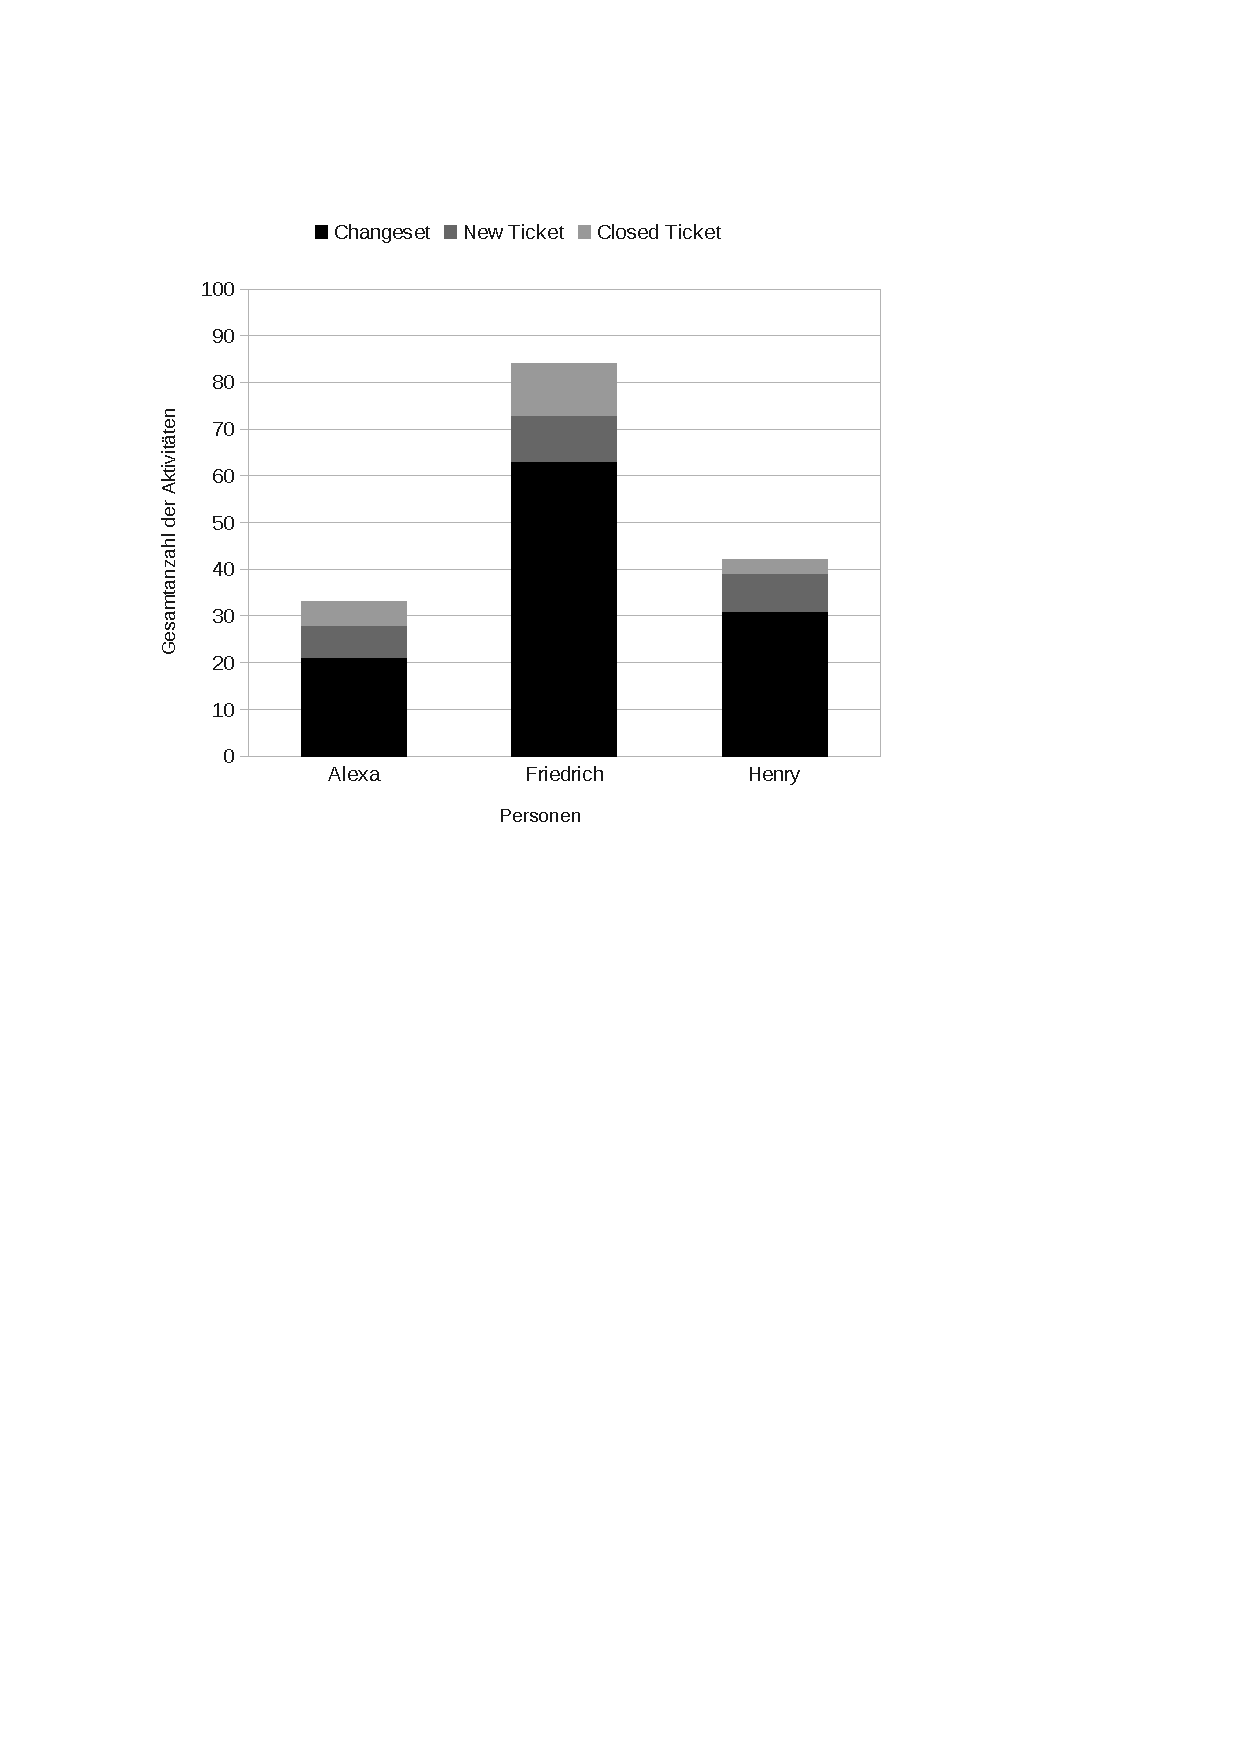
\includegraphics{03_pics/stat1.pdf}
\caption{Aktivität pro Person}
\label{fig:activePP}
\end{figure}

\begin{figure}[htbp]
\centering
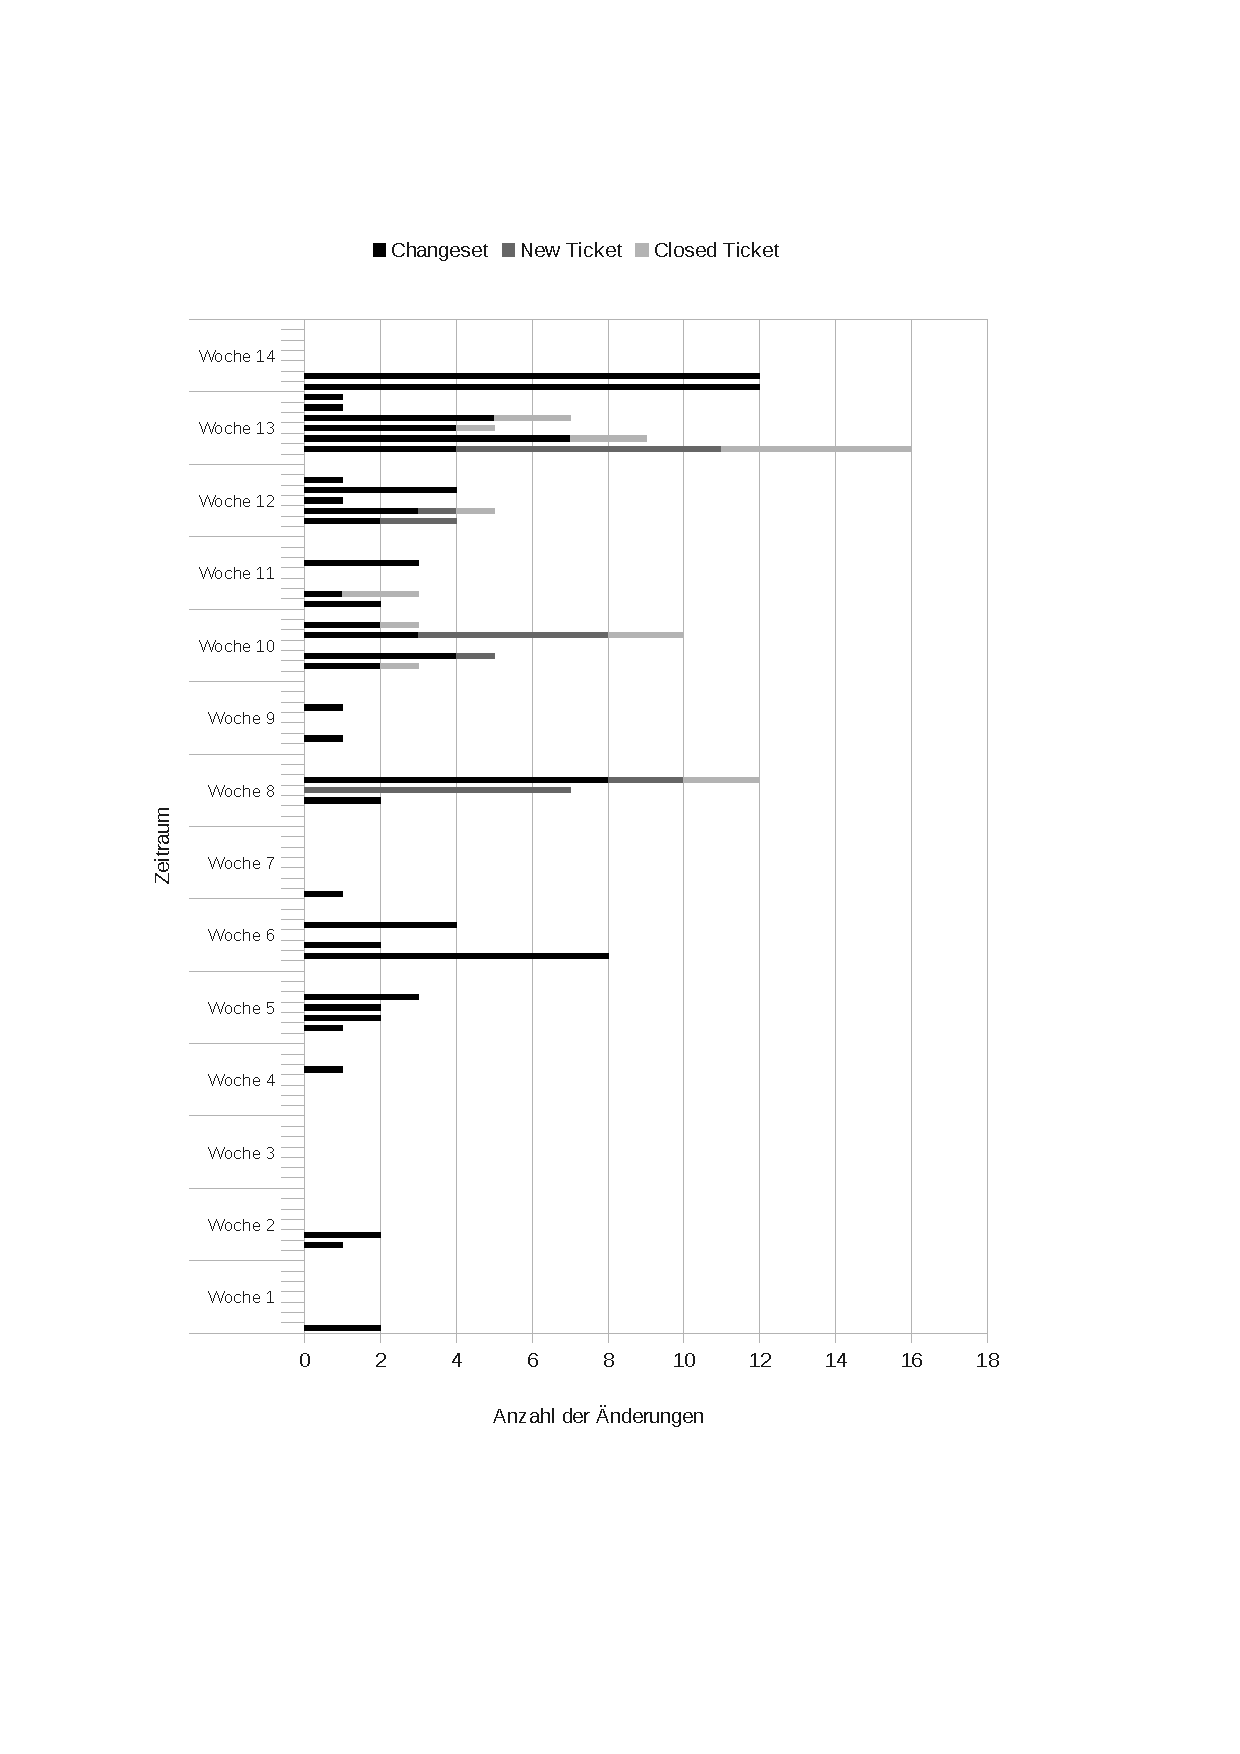
\includegraphics{03_pics/stat2.pdf}
\caption{Timeline}
\label{fig:activeTime}
\end{figure}


%%%%%%%%%%%%%%%%%%%%%%%%%%%%%%%%%%%%%%%%%%%%%%%%%%%%%%%%%%%%%%%%%%%%%%%%%%%%%%%
%%%%%%%%%%%%%%%%%%%%%%%%%%%%%%%%%%%%%%%%%%%%%%%%%%%%%%%%%%%%%%%%%%%%%%%%%%%%%%%
%%%%%%%%%%%%%%%%%%%%%%%%%%%%%%%%%%%%%%%%%%%%%%%%%%%%%%%%%%%%%%%%%%%%%%%%%%%%%%%
% FAZIT %%%%%%%%%%%%%%%%%%%%%%%%%%%%%%%%%%%%%%%%%%%%%%%%%%%%%%%%%%%%%%%%%%%%%%%
%%%%%%%%%%%%%%%%%%%%%%%%%%%%%%%%%%%%%%%%%%%%%%%%%%%%%%%%%%%%%%%%%%%%%%%%%%%%%%%
\subsection{Fazit zum Projektmanagement}
\label{subsec:fazitPM}

Für unser Softwareprojekt war unser Vorgehen als Gruppe nicht sehr optimal, hat aber trotzdem am Ende zu einem guten und lauffähigen Programm geführt. Trotzdem würden wir als Gruppe in einem neuen Projekt viele Dinge anders gestalten.

Ein erster Punkt wäre die Auswahl der Programmiersprache, wobei wir beim nächsten Mal eine Sprache wählen wollen, welche alle Teammitglieder ausreichend gut beherrschen, beispielsweise \emph{Java}. Diese Entscheidung würde unser radikales Vorgehen etwas entradikalisieren. Das Erstellen eines Zeitplans mit Meilensteinen und Arbeitspaketen ist ein Muss für das nächste Projekt.
Das Einsetzen eines Teamleiters, welcher nach außen hin die Kommunikation mit dem Professor und anderen Teams übernimmt und sich um die Organisation von Teamtreffen kümmert ist erstrebenswert. Um die Arbeitsmoral stets angenehm und positiv zu halten würden wir \emph{Coding Sessions} einplanen, wo sich alle Teammitglieder an einem Ort zum Programmieren treffen. Regelmäßige Protokolle sollten abwesenden Mitgliedern helfen auf dem aktuellen Stand der Entwicklung zu bleiben und Designentscheidungen nachzuvollziehen.
Wir haben darüber nachgedacht ein konkretes Vorgehensmodell zur Softwareentwicklung einzusetzen, beispielsweise \emph{Scrum}.
\clearpage

\section{Bedienungsanleitung und GUI}
\label{sec:frontend}

Im Folgenden wir die Installation und die Bedienung des Programms erläutert, sowie der Aufbau der Oberfläche beschrieben. Das Programm kann unter \url{https://dev.spline.de/svn/CommonUnfold/trunk/} runter geladen\footnote{\texttt{\$ svn checkout \url{https://dev.spline.de/svn/CommonUnfold/trunk/}}} werden. Im Ordner \texttt{src} muss die Datei \texttt{common\_unfolding\_draw.py} mit dem folgenden Befehl gestartet werden:\\

\centerline{\texttt{\$ python common\_unfolding\_draw.py\\[2ex]}}


Wird das Programm gestartet, so befindet man sich im Startfenster (siehe~Abb.~\ref{fig:startFenster}). Über den Menüeintrag \texttt{File} können neue Schachteln erzeugt (\texttt{New By Surface, New By Dimension}) oder gespeicherte Arbeiten geöffnet werden (\texttt{Open File - Ctrl+O}).

\begin{figure}[htbp]
  \centering
  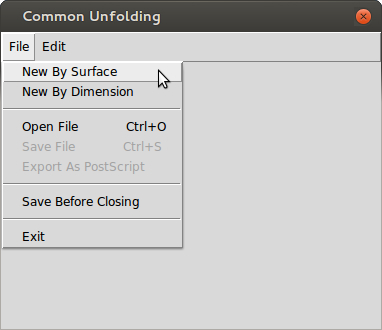
\includegraphics[scale=0.5]{03_pics/start.jpg}
  \caption{Startfenster}
  \label{fig:startFenster}
\end{figure}


%%%%%%%%%%%%%%%%%%%%%%%%%%%%%%%%%%%%%%%%%%%%%%%%%%%%%%%%%%%%%%%%%%%%%%%%%%%%%%%
%%%%%%%%%%%%%%%%%%%%%%%%%%%%%%%%%%%%%%%%%%%%%%%%%%%%%%%%%%%%%%%%%%%%%%%%%%%%%%%
%%%%%%%%%%%%%%%%%%%%%%%%%%%%%%%%%%%%%%%%%%%%%%%%%%%%%%%%%%%%%%%%%%%%%%%%%%%%%%%
% SCHACHTELN ERZEUGEN %%%%%%%%%%%%%%%%%%%%%%%%%%%%%%%%%%%%%%%%%%%%%%%%%%%%%%%%%
%%%%%%%%%%%%%%%%%%%%%%%%%%%%%%%%%%%%%%%%%%%%%%%%%%%%%%%%%%%%%%%%%%%%%%%%%%%%%%%
\subsection{Erzeugen von Schachteln}
\label{subsec:schachteln}

Die Anzahl der Schachteln kann man beim Erzeugen von neuen Schachteln frei wählen, \dH es können auch mehr als zwei Grundflächen ausgewählt werden. Aus dem sich ergebenden Common-Unfold soll es möglich sein, die zuvor ausgewählten Schachteln zu falten. Bei der Erzeugung von neuen Schachteln, kann zwischen \texttt{New By Surface} und \texttt{New By Dimension} gewählt werden.

  \begin{description}
    \item [{New~By~Surface:}] Hier gibt man den Oberflächeninhalt an. Gibt es mehr als eine Schachtel, welche diesen Oberflächeninhalt hat, so werden diese erzeugt. Beispielsweise erzeugen die Oberflächeninhalte $22, 30, 34, 38, 40$ und $42$ jeweils zwei verschieden dimensionierte Schachteln, die Oberflächeninhalte $46, 54$ und $58$ jeweils drei Schachteln.

    \item [{New~By~Dimension:}] Hier gibt man die Breite, Höhe und Tiefe einer Schachtel an. Alle weiteren, die in die gleiche Äquivalenzklasse fallen, werden erzeugt. Funktionierende Beispiele dafür sind die Dimensionen $1\times1\times5$, $1\times2\times3$ und $1\times4\times5$.
  \end{description}

Alle Schachteln werden in einer \emph{Preview} angezeigt und stehen in einem neuen Fenster zur Auswahl (Checkboxen)  bereit (siehe~Abb.~\ref{fig:preview}). Man muss mindestens zwei Schachteln auswählen um das Programm zu starten. Existieren nur zwei Schachteln, werden diese automatisch vorausgewählt. Zusätzlich kann man die Rotation der Schachteln in Grad angeben, diese werden dabei um ihren Urspungspunkt im Uhrzeigersinn rotiert.

\begin{figure}[htbp]
  \centering
  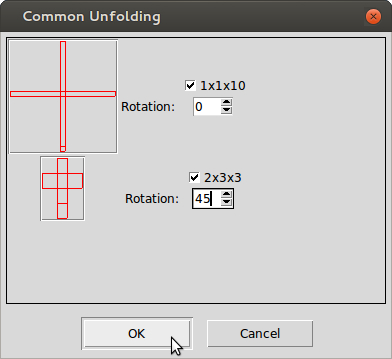
\includegraphics[scale=0.5]{03_pics/auswahl.jpg}
  \caption{Preview: Auswahlfenster für Schachteln}
  \label{fig:preview}
\end{figure}


%%%%%%%%%%%%%%%%%%%%%%%%%%%%%%%%%%%%%%%%%%%%%%%%%%%%%%%%%%%%%%%%%%%%%%%%%%%%%%%
%%%%%%%%%%%%%%%%%%%%%%%%%%%%%%%%%%%%%%%%%%%%%%%%%%%%%%%%%%%%%%%%%%%%%%%%%%%%%%%
%%%%%%%%%%%%%%%%%%%%%%%%%%%%%%%%%%%%%%%%%%%%%%%%%%%%%%%%%%%%%%%%%%%%%%%%%%%%%%%
% ZEICHENOBERFLÄCHE %%%%%%%%%%%%%%%%%%%%%%%%%%%%%%%%%%%%%%%%%%%%%%%%%%%%%%%%%%%
%%%%%%%%%%%%%%%%%%%%%%%%%%%%%%%%%%%%%%%%%%%%%%%%%%%%%%%%%%%%%%%%%%%%%%%%%%%%%%%
\subsection{Zeichenoberfläche und Startpunkte}
\label{subsec:zeichenoberflaeche}

Wählt man mehr als eine Schachtel aus und bestätigt die Auswahl mit \texttt{OK}, so gelangt man zur \emph{Zeichenoberfläche} (siehe~Abb.~\ref{fig:zeichenoberflaeche}).\\

Die Zeichenoberfläche besteht aus den folgenden vier Bereichen:

  \begin{description}
    \item [{(1)~Zeichenbereich:}] In diesem Bereich wird gezeichnet, hier entsteht die neue Grundfläche, aus der die links angezeigten Schachteln gefaltet werden können.

    \item [(2)~Netze~der~Schachteln:] Im linken Bereich der Oberfläche werden alle ausgewählten Gitternetze untereinander angezeigt. Wird auf der Zeichenfläche gemalt, so wird auf den Schachteln die ausgemalte Fläche angezeigt.

    \item [(3)~Startpunkte-Dialog:] Bevor man mit dem Zeichnen beginnt, können Startpunkte auf den einzelnen Schachteln gesetzt werden, dies kann in einem extra Fenster passieren (es wird beim Erstellen der Schachteln automatisch geöffnet), indem die genauen $(x,y)$-Werte für alle Schachteln eingegeben werden oder auch durch Klicken auf die Schachteln direkt im Bereich~(2). Das Setzen der Startpunkte kann auch über die Menüleiste \texttt{Edit $\rightarrow$ Set Start Points} erfolgen. Werden keine Startpunkte gesetzt, so werden die Default-Werte verwendet.

    \item [(4)~Werkzeugleiste] Hier können verschiedene Optionen bezüglich des Zeichenvorgangs eingestellt werden. Dazu gehören das Einstellen der Pinselgröße, Zeichenfarbe und Pinselform. Außerdem können die Optionen \texttt{Overwrite}, \texttt{Autofill} und \texttt{Continue} aktiviert werden. Diese Optionen werden im nun folgenden Abschnitt~\ref{subsec:zeichnen} erläutert.
  \end{description}

\begin{figure}[htbp]
  \centering
  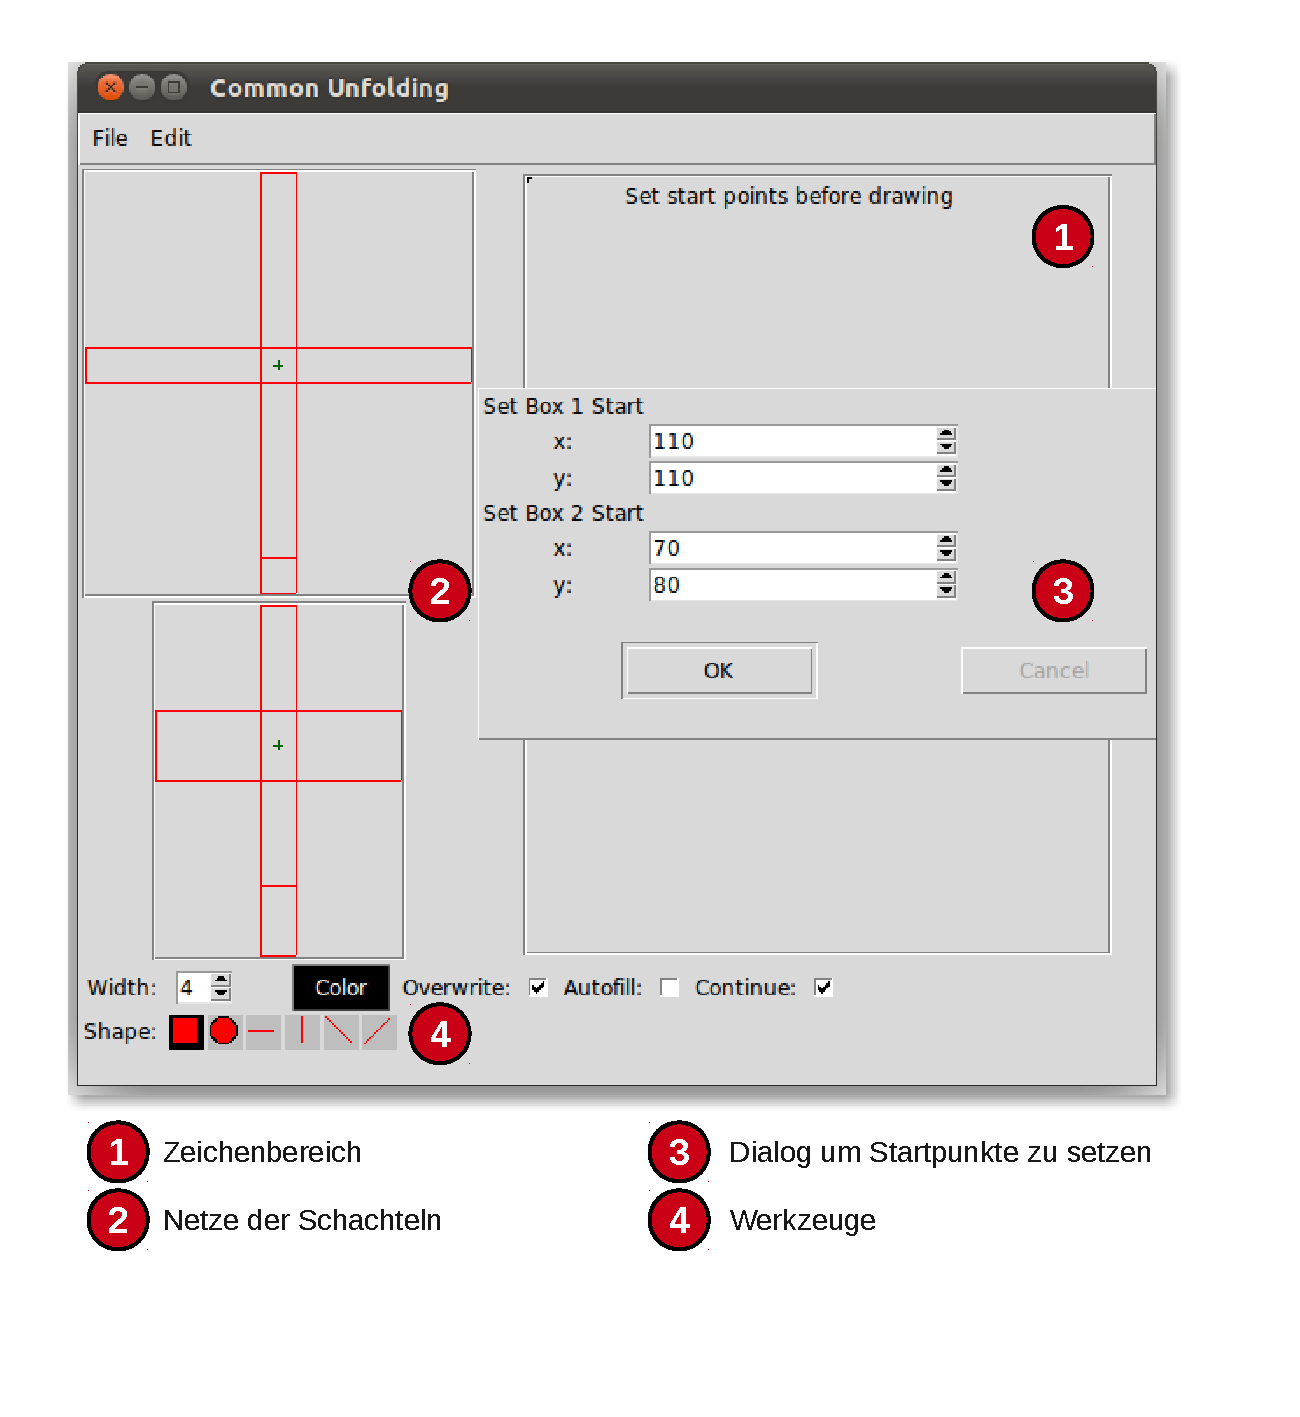
\includegraphics[scale=0.5]{03_pics/Zeichenbereich.pdf}
  \caption{Zeichenoberfläche}
  \label{fig:zeichenoberflaeche}
\end{figure}

%%%%%%%%%%%%%%%%%%%%%%%%%%%%%%%%%%%%%%%%%%%%%%%%%%%%%%%%%%%%%%%%%%%%%%%%%%%%%%%
%%%%%%%%%%%%%%%%%%%%%%%%%%%%%%%%%%%%%%%%%%%%%%%%%%%%%%%%%%%%%%%%%%%%%%%%%%%%%%%
%%%%%%%%%%%%%%%%%%%%%%%%%%%%%%%%%%%%%%%%%%%%%%%%%%%%%%%%%%%%%%%%%%%%%%%%%%%%%%%
% DAS ZEICHNEN %%%%%%%%%%%%%%%%%%%%%%%%%%%%%%%%%%%%%%%%%%%%%%%%%%%%%%%%%%%%%%%%
%%%%%%%%%%%%%%%%%%%%%%%%%%%%%%%%%%%%%%%%%%%%%%%%%%%%%%%%%%%%%%%%%%%%%%%%%%%%%%%
\subsection{Zeichnen}
\label{subsec:zeichnen}

Nachdem die Startpunkte gesetzt wurden, \bzw die Default-Werte übernommen wurden, kann im Zeichenbereich gezeichnet werden. Der erste Klick in den Zeichenbereich setzt den Ursprung des Rasters $(0,0)$. Zum Zeichnen klickt man einfach in den Zeichenbereich und hält die Maustaste gedrückt, der Curser wird zu einem Stift, mit welchem man malen kann. Es wird auf allen Oberflächen gleichzeitig gemalt. Die Position des Cursors wird mit Hilfe eines kleinen Kreuzes auf allen anderen Flächen angezeigt (siehe Abb.~\ref{fig:zeichnen}). Es kann auch auf den Schachtelflächen gemalt werden. Die Fläche die im Zeichenbereich entsteht sollte zusammenhängend sein.

\begin{figure}[htbp]
  \centering
  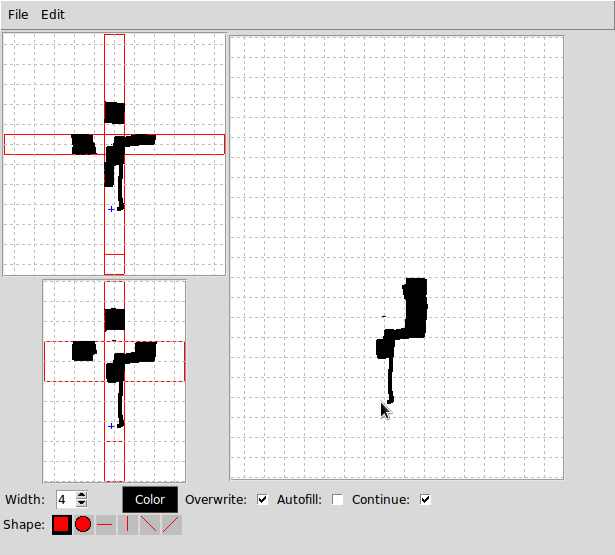
\includegraphics[scale=0.5]{03_pics/zeichnen.png}
  \caption{Zeichnen}
  \label{fig:zeichnen}
\end{figure}

Es können verschiedene Optionen über die Werkzeugleiste eingestellt werden, diese werde im Folgenden näher erläutert.

\begin{description}
  \item [Overwrite] Aktiviert man \texttt{Overwrite} so werden breits ausgemalte Flächenstücke überschrieben.

  \item [Autofill] In Kombination mit dem aktivierten \texttt{Overwrite} bewirkt \texttt{Autofill}, dass durch \texttt{Overrite} entstandene unausgemalte Flächenstücke automatisch aufgefüllt werden.

  \item [Continue] \texttt{Continue} ermöglicht, dass man von einer schon gezeichneten Fläche weitermalen kann und auf allen Flächen die richtige Richtung hat, so als ob man durchgehend gezeichnet hätte.
\end{description}


%%%%%%%%%%%%%%%%%%%%%%%%%%%%%%%%%%%%%%%%%%%%%%%%%%%%%%%%%%%%%%%%%%%%%%%%%%%%%%%
%%%%%%%%%%%%%%%%%%%%%%%%%%%%%%%%%%%%%%%%%%%%%%%%%%%%%%%%%%%%%%%%%%%%%%%%%%%%%%%
%%%%%%%%%%%%%%%%%%%%%%%%%%%%%%%%%%%%%%%%%%%%%%%%%%%%%%%%%%%%%%%%%%%%%%%%%%%%%%%
% LADEN, SPEICHERN, EXPORTIEREN %%%%%%%%%%%%%%%%%%%%%%%%%%%%%%%%%%%%%%%%%%%%%%%
%%%%%%%%%%%%%%%%%%%%%%%%%%%%%%%%%%%%%%%%%%%%%%%%%%%%%%%%%%%%%%%%%%%%%%%%%%%%%%%
\subsection{Menüleiste und Shortcuts}
\label{subsec:dateioperationen}

Über die Menüleiste können Dateien gespeichert, geladen und exportiert werden. Außerdem können Aktionen rückgängig gemacht und wiederholt werden, zudem kann die Option \texttt{Save Before Closing} aktiviert werden.

\begin{description}
  \item [Open File] Es können zuvor gespeicherte Dateien mit \texttt{Ctrl+O} geöffnet werden. Gespeicherte Dateien sind \texttt{CommonUnfoldFiles} mit der Dateiendung \texttt{*.cuf}.
  \item [Save File] Dateien können als \texttt{*.cuf} gespeichert werden.
  \item [Export As PostScript] Dateien können als PostScript (\texttt{*.ps}) exportiert werden. Gespeichert wird nur der Zeichenbereich (der Bereich auf der rechten Seite).
  \item [Save Before Closing] Diese Option kann aktiviert werden, so werden Dateien automatisch beim Schließen des Programms abgespeichert.
  \item [Undo] Mit \texttt{Ctrl+Z} können Schritte rückgängig gemacht werden.
  \item [Redo] Mit \texttt{Ctrl+Y} können Schritte wiederholt werden. 
\end{description}
\clearpage

\section{Softwarearchitektur}
\label{sec:backend}

In diesem Teil der Arbeit wird die technische Umsetzung des Projekts erläutert. Dazu gehören die funktionalen Anforderungen, welche zum größten Teil durch unsere Aufgabenstellung gegeben waren, sowie die Beschreibung der Funktionsweise des Programms. Auf Schwierigkeiten und Herausforderungen bezüglich der technischen Umsetzung und Algorithmen wird näher eingegangen.\\


%%%%%%%%%%%%%%%%%%%%%%%%%%%%%%%%%%%%%%%%%%%%%%%%%%%%%%%%%%%%%%%%%%%%%%%%%%%%%%%
%%%%%%%%%%%%%%%%%%%%%%%%%%%%%%%%%%%%%%%%%%%%%%%%%%%%%%%%%%%%%%%%%%%%%%%%%%%%%%%
%%%%%%%%%%%%%%%%%%%%%%%%%%%%%%%%%%%%%%%%%%%%%%%%%%%%%%%%%%%%%%%%%%%%%%%%%%%%%%%
% FUNKTIONALE ANFORDERUNGEN %%%%%%%%%%%%%%%%%%%%%%%%%%%%%%%%%%%%%%%%%%%%%%%%%%%
%%%%%%%%%%%%%%%%%%%%%%%%%%%%%%%%%%%%%%%%%%%%%%%%%%%%%%%%%%%%%%%%%%%%%%%%%%%%%%%
\subsection{Funktionale Anforderungen}
\label{subsec:anforderungen}

Im Fogenden werden wir die funktionalen Anforderungen an unser Programm erläutern. Diese waren vor allem durch die Aufgabenstellung gegeben. Ziel war es eine grafische Oberfläche zu entwickeln mit der es möglich ist das Konzept des simultanen Zeichnens zu verwenden.

\paragraph{Optionale Verknüpfung von Randstücken}
Wird ein Gitternetz eines Quaders gezeichnet, so entstehen doppelte Kanten, obwohl es diese Kanten nur einmal gibt. Hier galt es eine Regel zu finden um Ungenauigkeiten zu vermeiden.

\paragraph{Unterstützung der Anfangszuordnung}
Bevor mit dem Zeichnen begonnen wird, sollen die Startpunkte auf den einzelnen Schachteln ausgewählt werden können.

\paragraph{Automatisierung der Verarbeitung verschiedener Schachteln}
Es soll durch den Benutzer ausgewählt werden, welche Schachteln er bearbeiten möchte.

\paragraph{Automatisches Auffüllen}
Wird an einer Stelle etwas weggenommen, weil es zum Beispiel durch eine andere Fläche übermalt wurde, so sollen automatisch die Zwischenräume mit Farbe aufgefüllt werden.

%%%%%%%%%%%%%%%%%%%%%%%%%%%%%%%%%%%%%%%%%%%%%%%%%%%%%%%%%%%%%%%%%%%%%%%%%%%%%%%
%%%%%%%%%%%%%%%%%%%%%%%%%%%%%%%%%%%%%%%%%%%%%%%%%%%%%%%%%%%%%%%%%%%%%%%%%%%%%%%
%%%%%%%%%%%%%%%%%%%%%%%%%%%%%%%%%%%%%%%%%%%%%%%%%%%%%%%%%%%%%%%%%%%%%%%%%%%%%%%
% WEITERES AN FUNKTIONALITÄT %%%%%%%%%%%%%%%%%%%%%%%%%%%%%%%%%%%%%%%%%%%%%%%%%%
%%%%%%%%%%%%%%%%%%%%%%%%%%%%%%%%%%%%%%%%%%%%%%%%%%%%%%%%%%%%%%%%%%%%%%%%%%%%%%%
\subsection{Weitere Funktionalität}
\label{subsec:weiteres}

\begin{itemize}
  \item Zeichnen auch auf Schachteln
  \item Anzeigen der Curserposition
  \item Anzeigen eines Grids
  \item Undo/Redo
  \item Speichern/Laden
  \item Zeichendicke und Form
  \item Rotation
\end{itemize}

%%%%%%%%%%%%%%%%%%%%%%%%%%%%%%%%%%%%%%%%%%%%%%%%%%%%%%%%%%%%%%%%%%%%%%%%%%%%%%%
%%%%%%%%%%%%%%%%%%%%%%%%%%%%%%%%%%%%%%%%%%%%%%%%%%%%%%%%%%%%%%%%%%%%%%%%%%%%%%%
%%%%%%%%%%%%%%%%%%%%%%%%%%%%%%%%%%%%%%%%%%%%%%%%%%%%%%%%%%%%%%%%%%%%%%%%%%%%%%%
% FUNKTIONSWEISE %%%%%%%%%%%%%%%%%%%%%%%%%%%%%%%%%%%%%%%%%%%%%%%%%%%%%%%%%%%%%%
%%%%%%%%%%%%%%%%%%%%%%%%%%%%%%%%%%%%%%%%%%%%%%%%%%%%%%%%%%%%%%%%%%%%%%%%%%%%%%%
\subsection{Beschreibung der Funktionsweise}
\label{subsec:funktionsweise}

Alle Zeichenvorgänge gehen von einer Benutzereingabe auf der Hauptzeichenfläche aus, auch beim Zeichnen auf den Schachtel-Zeichenflächen wird ein entsprechendes Ereignis auf der Hauptfläche ausgelöst, welches in der draw-Methode des DrawingCanvas-Objektes behandelt wird.\\

Von den $x - $ und $y - $Koordinaten dieses Ereignisses ausgehend wird von jeder Schachtel-Zeichenfläche die Funktion \texttt{prepare(x, y)} aufgerufen.\\

In den Zeichenflächen werden die Koordinaten berechnet, die beim aktuellen Zeichenvorgang dem Punkt auf der Hauptfläche entsprechen. Zusätzlich wird angegeben, ob dieser Punkt auf der Schachtel-Zeichenfläche bereits existiert. Falls es auf einer Fläche nicht möglich sein sollte, entsprechende Koordinaten zu berechnen, wird der Zeichenvorgang abgebrochen.\\

Falls in den berechneten Schachtel-Koordinaten Konflikte aufgetreten sind, also Punkte auf den Schachtelflächen bereits vorhanden sind, und das Überschreiben aktiviert ist, werden die bereits vorhandenen Punkte und ihre entsprechenden Punkte auf den anderen Zeichenflächen gelöscht. Ein auf der Hauptzeichenfläche bereits vorhandener Punkt wird ebenso behandelt. Sollte \emph{Überschreiben} nicht aktiviert sein, muss der Zeichenvorgang bei vorhandenen Konflikten abgebrochen werden.\\

Nachdem nun mögliche Konflikte behoben sind,, können alle berechneten Punkte gezeichnet werden.\\


%%%%%%%%%%%%%%%%%%%%%%%%%%%%%%%%%%%%%%%%%%%%%%%%%%%%%%%%%%%%%%%%%%%%%%%%%%%%%%%
% SCHACHTEL KOORDINATEN %%%%%%%%%%%%%%%%%%%%%%%%%%%%%%%%%%%%%%%%%%%%%%%%%%%%%%%
%%%%%%%%%%%%%%%%%%%%%%%%%%%%%%%%%%%%%%%%%%%%%%%%%%%%%%%%%%%%%%%%%%%%%%%%%%%%%%%
\subsubsection{Berechnen der Schachtel-Koordinaten}
\label{subsubsec:schachtelkoordinaten}

In der Funktion \texttt{prepare(x, y)} der BoxCanvas-Objekte wird von den $x$-, $y$-Koordinaten der Hauptzeichenfläche ausgehend die Koordinaten des entsprechenden Punktes der Schachtel-Zeichenfläche berechnet.\\

Ausgehend vom Startpunkt der Schachtelfläche wird eine Verschiebung der Koordinaten addiert. Falls z. B. der Startpunkt der Hauptfläche $(100|100)$ ist und der Startpunkt der Schachtelfläche $(200|300)$, so ergibt sich $(x+100|y+200)$.\\

Zu jeder Schachtelfläche gehört eine Liste \texttt{traversed\_edges}, in der die im aktuellen Zeichenvorgang überquerten Kanten gespeichert werden. Nun wird nacheinander die traverse-Funktion der Kanten für die $x$-, $y$-Koordinaten aufgerufen.\\

Nun muss festgestellt werden, ob der berechnete Punkt wiederum außerhalb der Schachtel liegt, ob also eine weitere Kante überquert wurde, oder ob der Punkt innerhalb der Schachtel liegt. Dazu werden Orientierungstest mit den Eckpunkten der beiden Rechtecke, die die Schachtelfläche bilden ausgeführt (Funktion \texttt{is\_inside(x, y)}).\\

Falls der Punkt außerhalb liegt und im aktuellen Zeichenvorgang bereits ein Punkt gezeichnet wurde, also ein gültiger Referenzpunkt vorliegt, wird die zwischen den beiden Punkten liegende Kante festgestellt. Für diese Kante wird ebenfalls die traverse-Funktion aufgerufen, wodurch wir wiederum neue Koordinaten erhalten.\\

Falls kein Referenzpunkt vorhanden ist, kann kein gültiger Punkt berechnet werden.\\

Nun haben wir also gültige Koordinaten für einen auf der Schachtel liegenden Punkt und möglicherweise eine neu überquerte Kante (sollte der Punkt schließlich gezeichnet werden, wird diese Kante zur Liste der Überquerten hinzugefügt). Jetzt wird noch geprüft ob der berechnete Punkt bereits gezeichnet wurde. Diese Information wird zusammen mit den berechneten Koordinaten zurückgegeben.\\


%%%%%%%%%%%%%%%%%%%%%%%%%%%%%%%%%%%%%%%%%%%%%%%%%%%%%%%%%%%%%%%%%%%%%%%%%%%%%%%
% AUTOMATISCHES AUFFÜLLEN %%%%%%%%%%%%%%%%%%%%%%%%%%%%%%%%%%%%%%%%%%%%%%%%%%%%%
%%%%%%%%%%%%%%%%%%%%%%%%%%%%%%%%%%%%%%%%%%%%%%%%%%%%%%%%%%%%%%%%%%%%%%%%%%%%%%%
\subsubsection{Automatisches Auffüllen}
\label{subsubsec:auffuellen}

Falls auf einer Schachtelfläche ein Punkt gelöscht wird (z. B. aufgrund von Überschreibung), wird dieser Löschvorgang gespeichert. Nachdem der aktuelle Punkt gezeichnet wurde, werden die gelöschten Punkt überprüft. Falls ein Punkt tatsächlich gelöscht wurde, also kein neuer Punkt an der gleichen Stelle gezeichnet wurde, wird in der Funktion \texttt{get\_autofill} geprüft, ob auf der entsprechenden Zeichenfläche in der näheren Umgebung bereits gezeichnet wurde. Die Anzahl der überprüften Pixel ist abhängig von der eingestellten Zeichenbreite.\\

Falls ein entsprechender Punkt gefunden wird, wird von diesem aus "`aufgefüllt"'. Der gelöschte Punkt wird also so gezeichnet, als wäre er im gleichen Zeichenvorgang entstanden wie der bereits vorhandene Punkt.\\ 


%%%%%%%%%%%%%%%%%%%%%%%%%%%%%%%%%%%%%%%%%%%%%%%%%%%%%%%%%%%%%%%%%%%%%%%%%%%%%%%
% STARTPUNKTE %%%%%%%%%%%%%%%%%%%%%%%%%%%%%%%%%%%%%%%%%%%%%%%%%%%%%%%%%%%%%%%%%
%%%%%%%%%%%%%%%%%%%%%%%%%%%%%%%%%%%%%%%%%%%%%%%%%%%%%%%%%%%%%%%%%%%%%%%%%%%%%%%
\subsubsection{Setzen von Startpunkten}
\label{subsubsec:startpunkte}
Startpunkte werden für jede Schachtelflächen gesetzt. Diese Werte werden als Offset in \texttt{box\_canvas.offset} gespeichert. Wird der Startpunkt auf der Zeichenfläche gesetzt, so wird dieser von allen \texttt{box\_canvas.offset}`s subtrahiert.


%%%%%%%%%%%%%%%%%%%%%%%%%%%%%%%%%%%%%%%%%%%%%%%%%%%%%%%%%%%%%%%%%%%%%%%%%%%%%%%
% UNDO/REDO %%%%%%%%%%%%%%%%%%%%%%%%%%%%%%%%%%%%%%%%%%%%%%%%%%%%%%%%%%%%%%%%%%%
%%%%%%%%%%%%%%%%%%%%%%%%%%%%%%%%%%%%%%%%%%%%%%%%%%%%%%%%%%%%%%%%%%%%%%%%%%%%%%%
\subsubsection{Undo und Redo}
\label{subsubsec:undoRedo}

Beim Zeichenvorgang werdne alle Punkte in der Form $(x,y)$ gespeichert. Wenn ein vorher gezeichneter Punkt gelöscht wird, so werden alle dazugehörigen Punkte auf den einzelnen Boxen und der Zeichenfläche gespeichert. Zusätzlich wird der Anfangsstatus gespeichert. Dazu gehören die Zustände: \texttt{overwrite}, \texttt{autofill}, \texttt{continue} und die anfangs überquerten Kanten auf den Schachtelflächen.\\

Bei \texttt{Undo} werden alle diese Punkte mit \texttt{drawing\_canvas.erase} gelöscht und in der Redo-Liste gespeichert. Anschließend werden die durch diese gelöschten Punkt vorher überschriebenen Punkte wiederhergestellt\\

Bei \texttt{Redo} wird ein erneutes Zeichnen auf der Zeichenfläche mit Hilfe
von \texttt{my\_event} simuliert.\\


%%%%%%%%%%%%%%%%%%%%%%%%%%%%%%%%%%%%%%%%%%%%%%%%%%%%%%%%%%%%%%%%%%%%%%%%%%%%%%%
% SPEICHERN/LADEN %%%%%%%%%%%%%%%%%%%%%%%%%%%%%%%%%%%%%%%%%%%%%%%%%%%%%%%%%%%%%
%%%%%%%%%%%%%%%%%%%%%%%%%%%%%%%%%%%%%%%%%%%%%%%%%%%%%%%%%%%%%%%%%%%%%%%%%%%%%%%
\subsubsection{Speichern und Laden}
\label{subsubsec:speichernLaden}
Wird der Status einer Zeichenfläche abgespeichert, so wird eine modifzierte Undo-Liste als CommonUnfoldFile (\texttt{*.cuf}) abgespeichert.\\

Struktur des CommonUnfoldFiles:

\begin{itemize}
\item Integer: Anzahl der Schachteln
\item Quadtrupel für jede Schachtel: (Höhe, Breite, Tiefe, Rotation)
\item Tupel für jede Schachtel: Startpunkt der Schachtel $(x,y)$
\item Tupel: Startpunkt der Zeichenfläche $(x,y)$
\item Integer: Anzahl der gezeichneten Linien (Linie endet nach dem Loslassen der Maus)
\item Für jede Linie:
  \begin{itemize}
    \item Integer: Anzahl der Pixel
    \item Boolean: war der Status \texttt{overwrite} aktiv
    \item Boolean: war der Status \texttt{autofill} aktiv
    \item Boolean: war der Status \texttt{continue} aktiv
    \item Liste von Kanten für jede Schachtel (als Start \texttt{boxes.traversed}
    \item Tripel für jeden Pixel der Linie: $(x, y, Farbe)$
  \end{itemize}
\end{itemize}

Beim Laden einer \texttt{*.cuf} Datei, werden erst die Schachteln erstellt, dann die Startpunkte gesetzt und im Anschluss das Zeichnen simuliert.


%%%%%%%%%%%%%%%%%%%%%%%%%%%%%%%%%%%%%%%%%%%%%%%%%%%%%%%%%%%%%%%%%%%%%%%%%%%%%%%
% CURSOR %%%%%%%%%%%%%%%%%%%%%%%%%%%%%%%%%%%%%%%%%%%%%%%%%%%%%%%%%%%%%%%%%%%%%%
%%%%%%%%%%%%%%%%%%%%%%%%%%%%%%%%%%%%%%%%%%%%%%%%%%%%%%%%%%%%%%%%%%%%%%%%%%%%%%%
\subsubsection{Cursor}
\label{subsubsec:cursor}

Zeichnet man auf der Zeichenfläche wird gleichzeitig auf allen Schachteln die Postion der Maus mit Hilfe eines kleinen Kreuzes angezeigt. Befindet man sich mit der Maus auf einer Schachtel so wird auch diese Position auf allen anderen Schachteln und der Zeichenfläche angezeigt.
(1) Befindet man sich mit der Maus auf der Zeichenfläche so werden die Kreuze auf den Schachteln mit Hilfe eines Offsets berechnet und erstellt.
(2) Befindet man sich auf einer Schachtel, so wird der eigene Offset von der aktuellen Position abgezogen und das Kreuz auf der Zeichenfläche erstellt. Alle weiteren Kreuze auf den anderen Schachteln werden nun mit Methode (1) errechnet.


%%%%%%%%%%%%%%%%%%%%%%%%%%%%%%%%%%%%%%%%%%%%%%%%%%%%%%%%%%%%%%%%%%%%%%%%%%%%%%%
% CURSOR %%%%%%%%%%%%%%%%%%%%%%%%%%%%%%%%%%%%%%%%%%%%%%%%%%%%%%%%%%%%%%%%%%%%%%
%%%%%%%%%%%%%%%%%%%%%%%%%%%%%%%%%%%%%%%%%%%%%%%%%%%%%%%%%%%%%%%%%%%%%%%%%%%%%%%
\subsubsection{Zeichnen auf den Schachteln}
\label{subsubsec:zeichnenaufbox}

Zusaätzlich zum normalen Zeichen auf der Zeichenfläche kann auf den einzelnen Schachteln auch gezeichnet werden. Die Position auf der Schachtel wird auf die Position auf der Zeichenfläche umgerechten und dort wird dann die standardmäßige Draw-Funktion aufgerufen.


%%%%%%%%%%%%%%%%%%%%%%%%%%%%%%%%%%%%%%%%%%%%%%%%%%%%%%%%%%%%%%%%%%%%%%%%%%%%%%%
% ZEICHENDICKE UND FORM %%%%%%%%%%%%%%%%%%%%%%%%%%%%%%%%%%%%%%%%%%%%%%%%%%%%%%%
%%%%%%%%%%%%%%%%%%%%%%%%%%%%%%%%%%%%%%%%%%%%%%%%%%%%%%%%%%%%%%%%%%%%%%%%%%%%%%%
\subsubsection{Zeichendicke und Form}
\label{subsubsec:zeichendickeForm}

Für jeden Punkt der Fläche wird \texttt{draw} aufgerufen.
[TODO:XXX]


%%%%%%%%%%%%%%%%%%%%%%%%%%%%%%%%%%%%%%%%%%%%%%%%%%%%%%%%%%%%%%%%%%%%%%%%%%%%%%%
% GENERIEUNG VON SCHACHTELN UND PREVIEW %%%%%%%%%%%%%%%%%%%%%%%%%%%%%%%%%%%%%%%
%%%%%%%%%%%%%%%%%%%%%%%%%%%%%%%%%%%%%%%%%%%%%%%%%%%%%%%%%%%%%%%%%%%%%%%%%%%%%%%
\subsubsection{Generierung der Schachteln}
\label{subsubsec:generierungPreview}
Schachteln werden immer über den Flächeninhalt erzeugt. Ist die Dimension einer Schachtel gegeben, so wird im ersten Schritt der Oberflächeninhal (\texttt{calc\_surface\_area} berechnet. Im zweiten Schritt werden alle Schachteln $(a\times b \times c)$ berechnet, welche den gleichen Oberflächeninhalt haben.

\begin{lstlisting}[caption=Generierung von Schachteln]
# Calculates the surfaceare by edgelenght a,b,c
def calc_surface_area (a, b, c):
  return 2 * a * b + 2 * a * c + 2 * b * c

# Input: surfacearea of a cuboid
# Returs: all tupel (a,b,c), where a,b,c are the edgelenght beeing in that same equivalence relation
def create_triple(surface):
  surface = surface/2
  tripelList = []
  for a in range(1, int(sqrt(surface // 3)) + 1):
    b = a
    c, rem = divmod(surface - a * b, a + b)
    while (c >= b):
      if rem == 0:
        tripelList.append((a, b, c, 0)) 
      b = b + 1
      c, rem = divmod(surface - a * b, a + b)
  
  return tripelList
\end{lstlisting}
\clearpage

\section{Zusammenfassung und Ausblick}
\label{sec:zusammenfassung}

%%%%%%%%%%%%%%%%%%%%%%%%%%%%%%%%%%%%%%%%%%%%%%%%%%%%%%%%%%%%%%%%%%%%%%%%%%%%%%%
%%%%%%%%%%%%%%%%%%%%%%%%%%%%%%%%%%%%%%%%%%%%%%%%%%%%%%%%%%%%%%%%%%%%%%%%%%%%%%%
%%%%%%%%%%%%%%%%%%%%%%%%%%%%%%%%%%%%%%%%%%%%%%%%%%%%%%%%%%%%%%%%%%%%%%%%%%%%%%%
% ERGEBNISSE DES SOFTWAREPROJEKTES %%%%%%%%%%%%%%%%%%%%%%%%%%%%%%%%%%%%%%%%%%%%
%%%%%%%%%%%%%%%%%%%%%%%%%%%%%%%%%%%%%%%%%%%%%%%%%%%%%%%%%%%%%%%%%%%%%%%%%%%%%%%
\subsection{Ergebnisse des Softwareprojekts}
\label{subsec:ergebnisse}

Haben wir unsere ursprünglichen Ziele erreicht? Was sind unsere Ergebinsse? Was wollten wir erreichen?

%%%%%%%%%%%%%%%%%%%%%%%%%%%%%%%%%%%%%%%%%%%%%%%%%%%%%%%%%%%%%%%%%%%%%%%%%%%%%%%
%%%%%%%%%%%%%%%%%%%%%%%%%%%%%%%%%%%%%%%%%%%%%%%%%%%%%%%%%%%%%%%%%%%%%%%%%%%%%%%
%%%%%%%%%%%%%%%%%%%%%%%%%%%%%%%%%%%%%%%%%%%%%%%%%%%%%%%%%%%%%%%%%%%%%%%%%%%%%%%
% ELESSONS LEARNED %%%%%%%%%%%%%%%%%%%%%%%%%%%%%%%%%%%%%%%%%%%%%%%%%%%%%%%%%%%%
%%%%%%%%%%%%%%%%%%%%%%%%%%%%%%%%%%%%%%%%%%%%%%%%%%%%%%%%%%%%%%%%%%%%%%%%%%%%%%%
\subsection{Lessons Learned}
\label{subsec:lessons}

Was haben wir bei dem Projekt gelernt?

%%%%%%%%%%%%%%%%%%%%%%%%%%%%%%%%%%%%%%%%%%%%%%%%%%%%%%%%%%%%%%%%%%%%%%%%%%%%%%%
%%%%%%%%%%%%%%%%%%%%%%%%%%%%%%%%%%%%%%%%%%%%%%%%%%%%%%%%%%%%%%%%%%%%%%%%%%%%%%%
%%%%%%%%%%%%%%%%%%%%%%%%%%%%%%%%%%%%%%%%%%%%%%%%%%%%%%%%%%%%%%%%%%%%%%%%%%%%%%%
% AUSBLICK %%%%%%%%%%%%%%%%%%%%%%%%%%%%%%%%%%%%%%%%%%%%%%%%%%%%%%%%%%%%%%%%%%%%
%%%%%%%%%%%%%%%%%%%%%%%%%%%%%%%%%%%%%%%%%%%%%%%%%%%%%%%%%%%%%%%%%%%%%%%%%%%%%%%
\subsection{Ausblick}
\label{subsec:ausblick}

Was könnten wir noch machen, welche Features brauchen wir noch, damit das Programm noch besser wird?
\clearpage







\nocite{*} 
\bibliographystyle{alexaAlpha}
\bibliography{refs}
\addcontentsline{toc}{section}{Literatur}

\clearpage


\listoffigures
\addcontentsline{toc}{section}{Abbildungsverzeichnis}
\clearpage

\listoftables
\addcontentsline{toc}{section}{Tabellenverzeichnis}

\end{document}